\section{Networking}

There are several network architectures, including:
\begin{enumerate}
    \item \textit{Monolithic app}: uses minimal network resources and proprietary protocols.
    \item \textit{Client-server}: involves high network demands within enterprise applications.
    \item \textit{Web applications}: utilizes ubiquitous TCP/IP, accessible from anywhere.
    \item \textit{Microservices}: cloud providers segment servers into microservices.
\end{enumerate}
Data center applications may include cloud computing, cloud storage, and web services, which help consolidate computation and network resources.

As server performance improves, the demand for inter-server bandwidth naturally increases. 
Doubling the number of compute or storage elements can easily double the aggregate compute capacity or storage. 
However, networking presents challenges for straightforward horizontal scaling. 
While doubling leaf bandwidth is straightforward, increasing bisection bandwidth is more complex, especially when every server needs to communicate with every other server.
\begin{definition}[\textit{Bisection bandwidth}]
    Bisection bandwidth refers to the bandwidth across the narrowest line that evenly divides the cluster into two parts.
\end{definition}
Bisection bandwidth characterizes network capacity, representing the ability of randomly communicating processors to transmit data across the network's central portion. 
Ensuring every server can communicate with every other server necessitates doubling not only the leaf bandwidth but also the bisection bandwidth.

To simplify scaling, several networking architectures can be employed:
\begin{itemize}
    \item \textit{Switch-centric}: utilizes switches for packet forwarding tasks.
    \item \textit{Server-centric}: employs servers equipped with multiple Network Interface Cards (NICs) to serve as switches alongside their computational functions.
    \item \textit{Hybrid}: combines elements of both switch-centric and server-centric architectures.
\end{itemize}

\subsection{Switch-centric architecture}
In switch-centric architectures, traffic is divided into two main flows:
\begin{itemize}
\item \textit{Northbound-southbound}: Direct connection between the internet and servers.
\item \textit{East-west}: Inter-server communication within a data center, often for storage replication and VM migration.
\end{itemize}
East-west traffic typically surpasses northbound-southbound traffic in volume and significance within the data center environment.
\begin{figure}[H]
    \centering
    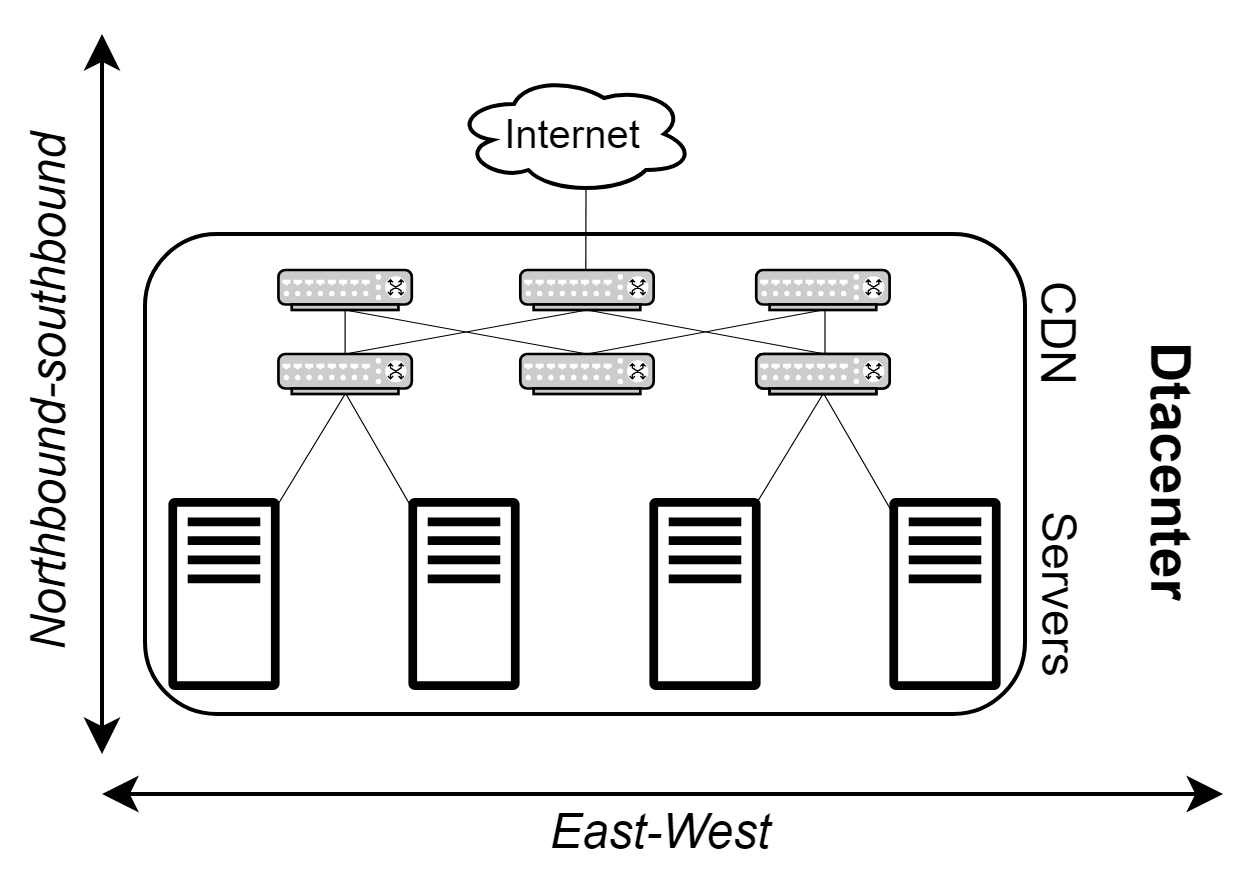
\includegraphics[width=0.6\linewidth]{images/sc.png}
    \caption{Switch-centric architecture}
\end{figure}

\paragraph*{Classical 3-tier architecture}
The classical 3-tier switch-centric architecture is structured into three distinct layers:
\begin{figure}[H]
    \centering
    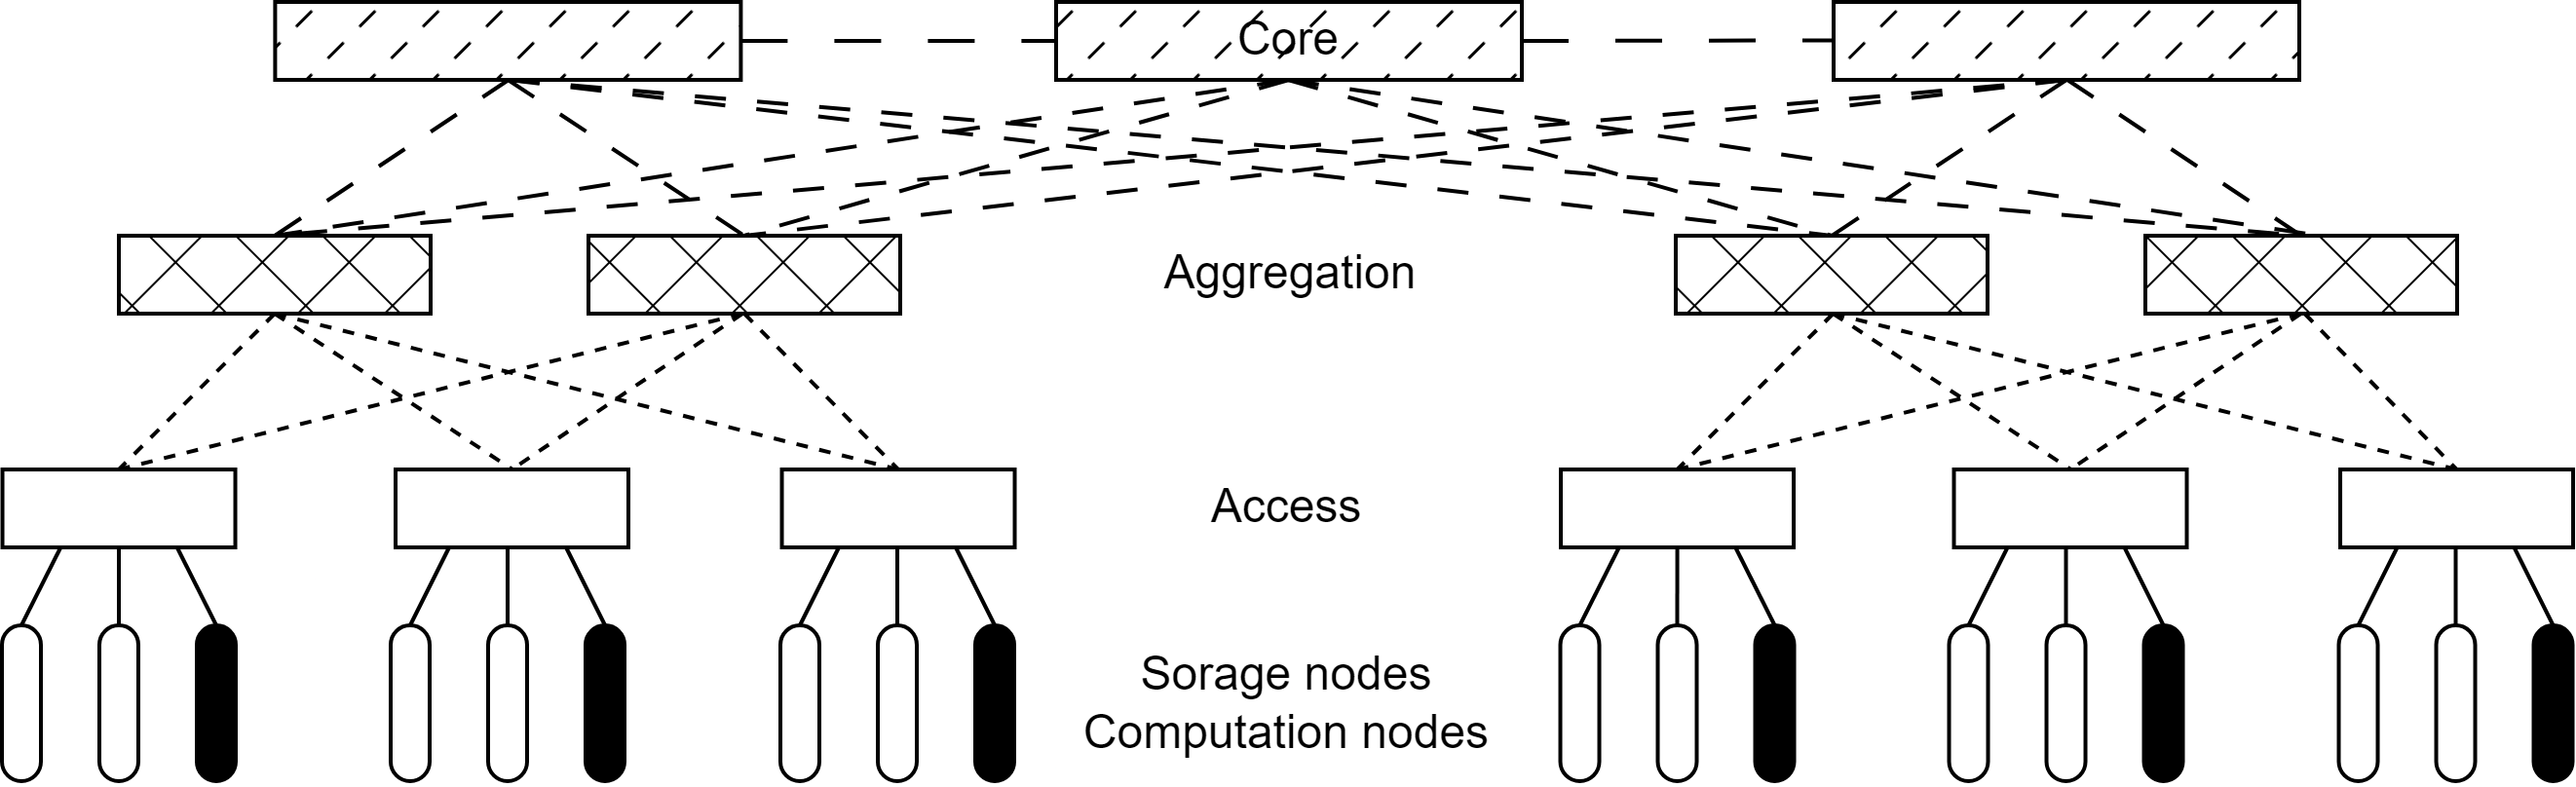
\includegraphics[width=0.75\linewidth]{images/sca.png}
    \caption{Classical 3-tier architecture} 
\end{figure}
In this configuration, servers interface with the Data Center Network (DCN) via access switches.

Switches can be categorized based on their position relative to the server racks:
\begin{itemize}
    \item \textit{Top-of-Rack} (ToR): all servers in a rack are linked to a ToR access switch. 
        Aggregation switches are housed either in dedicated racks or shared racks alongside other ToR switches and servers, resulting in simpler cabling and lower costs due to the limited number of ports per switch. 
        However, this configuration has limited scalability and increased switch management complexity.
    \item \textit{End-of-Row} (EoR): aggregation switches are placed at the end of each corridor, serving a row of racks. 
        Servers connect directly to the aggregation switch in another rack. 
        This arrangement requires more ports on the aggregation switches, more intricate cabling, and longer, costlier cables. 
        Typically, a patch panel facilitates connections between servers and the aggregation switch. 
        Despite more complex cabling, this setup offers simpler switch management.
\end{itemize}
Boosting bandwidth can be achieved through several methods. 
Increasing the number of switches at the core and aggregation layers enhances bandwidth. 
Additionally, using routing protocols like Equal Cost Multiple Path (ECMP) enables equitable traffic distribution across various routes, further enhancing bandwidth capabilities.

While this solution is straightforward, it can be costly in large data centers for several reasons. 
The upper layers require faster, more expensive network equipment, and each layer is serviced by different types of switches, increasing acquisition costs and complicating management, spare-part stocking, and energy consumption.

\paragraph*{Leaf-spine architecture}
The leaf-spine switch-centric architecture consists of two distinct layers:
\begin{itemize}
    \item \textit{Leaf}: ToR switch.
    \item \textit{Spine}: dedicated aggregation switches.
\end{itemize}
\begin{figure}[H]
    \centering
    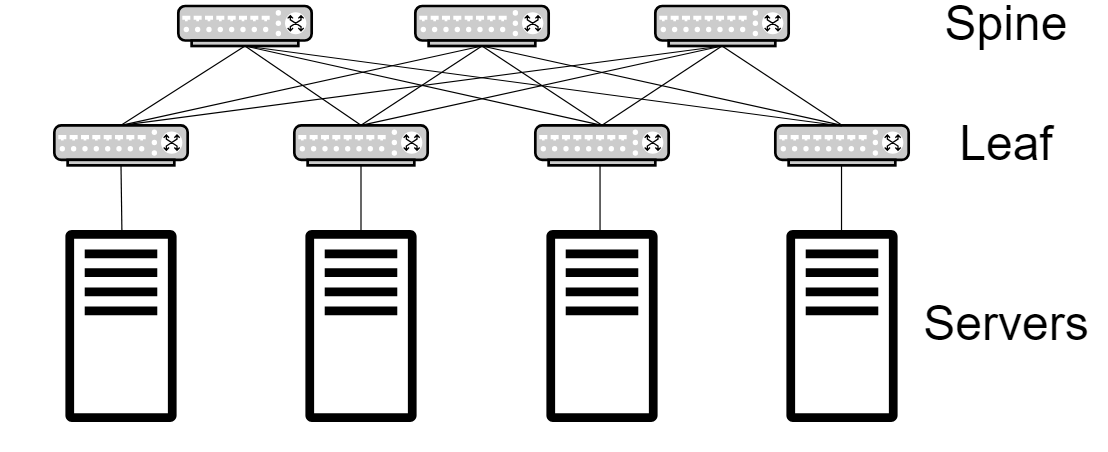
\includegraphics[width=0.6\linewidth]{images/ls.png}
    \caption{Leaf-spine architecture}
\end{figure}
Leaf-spine topologies are inspired by telephony networks, featuring a non-folded Clos structure. 
This architecture ensures that each stage is fully interconnected, with every matrix in one stage linked to every matrix in the subsequent stage.
\begin{figure}[H]
    \centering
    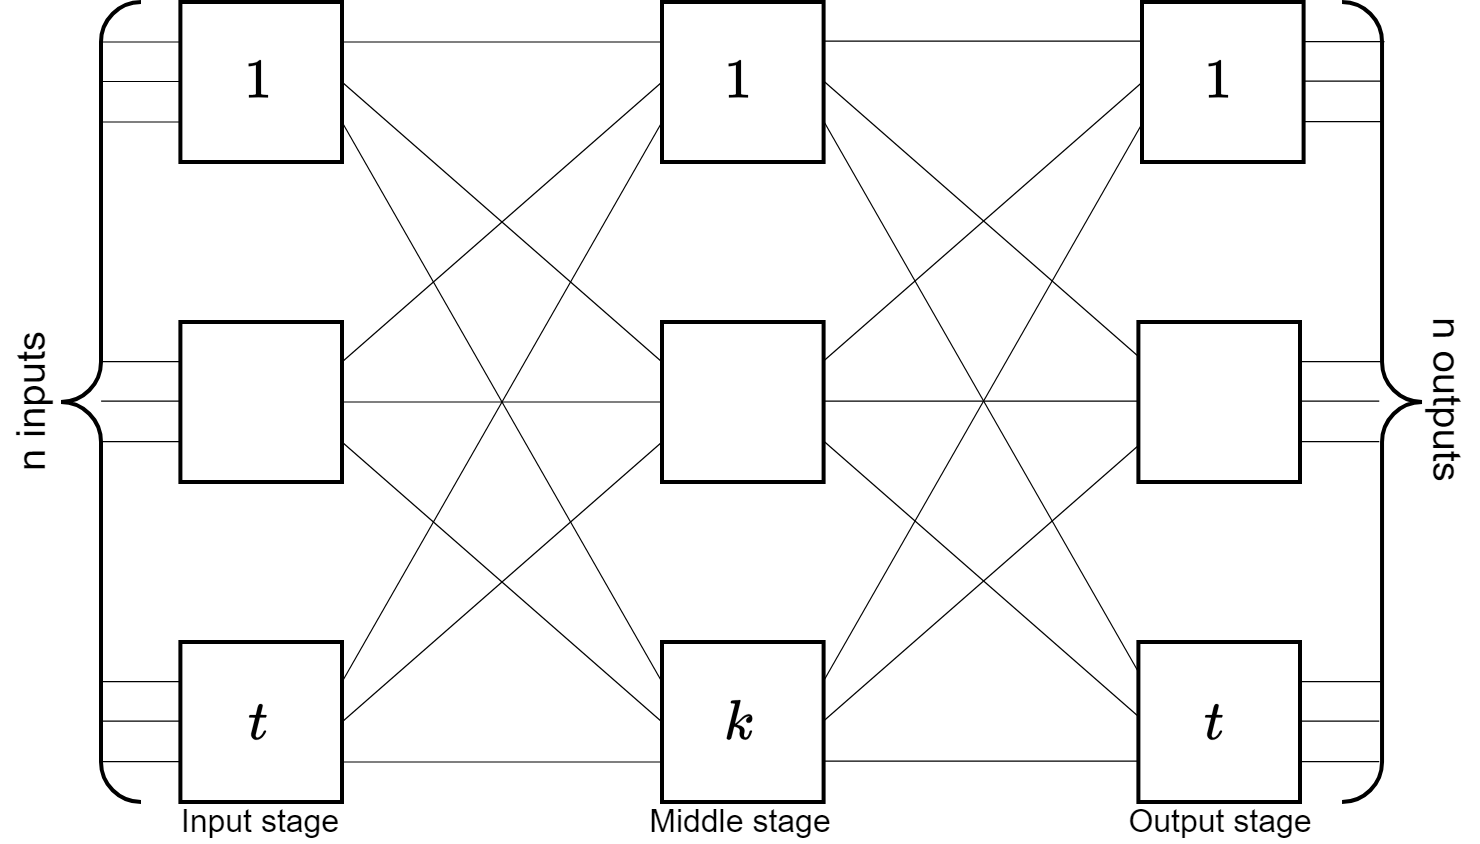
\includegraphics[width=0.6\linewidth]{images/stage.png}
    \caption{Clos network}
\end{figure}
When $k \geq n$, communication can always be reorganized to create a path between any pair of inactive input/output channels. 
If $k \geq 2n - 1$, a path between any pair of idle input/output channels is guaranteed to be available. 
The parameter $t$ is flexible in this topology, and when $n = t = k$, each switching module functions unidirectionally. 
In the leaf-spine topology, every switching module operates bidirectionally:
\begin{itemize}
    \item \textit{Leaf configuration}: comprises $t$ switching modules, each with $2k$ bidirectional ports per module.
    \item \textit{Spine configuration}: consists of $k$ switching modules, each with $t$ bidirectional ports.
\end{itemize}

The benefits of the leaf-spine architecture include:
\begin{itemize}
    \item Utilization of homogeneous equipment throughout the network, simplifying management and maintenance.
    \item Routing serves as the fundamental interconnect model, eliminating the need for Learning and Forwarding or Spanning Tree Protocol (STP).
    \item Implementation of Equal Cost Multiple Path (ECMP) strategy with routing protocols like IS-IS, SPB, or TRILL, enhancing network efficiency and resilience.
    \item Consistent number of hops for any pair of nodes, ensuring predictable and reliable communication.
    \item Small blast radius, minimizing the impact of network issues and failures.
\end{itemize}
To scale, a two-tier network structure can be expanded by introducing an additional row of switches or by transforming each spine-leaf group into a POD (Point of Delivery) and incorporating a super spine tier. 
This architecture represents a highly scalable and cost-effective DCN design.
\begin{figure}[H]
    \centering
    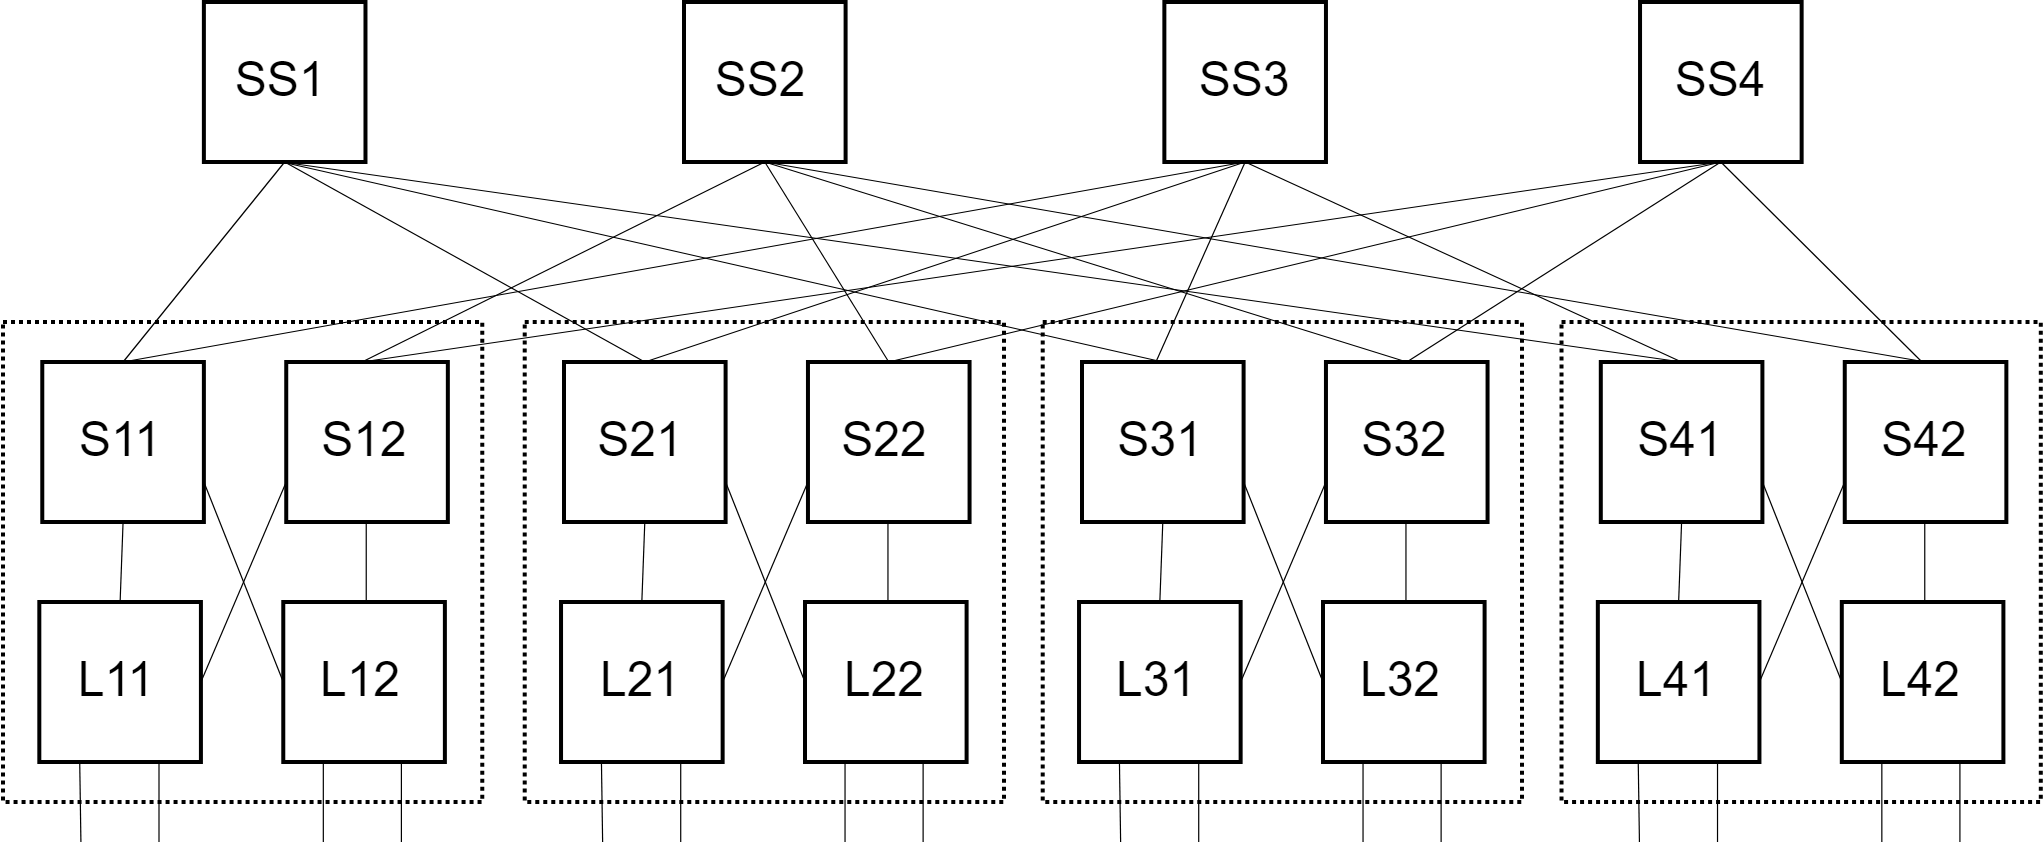
\includegraphics[width=0.6\linewidth]{images/pod.png}
    \caption{Pod-based three-tier Clos}
\end{figure}

A POD is a module or cluster comprising network, compute, storage, and application elements working together to provide a network service. 
The POD is a standardized and replicable pattern, enhancing the modularity, scalability, and manageability of data infrastructure.
A leaf switch with $2k^2$ bidirectional ports is configured with $k$ ports connecting to servers and $k$ ports linking to the DCN.
The POD is replicated $P$ times, each consisting of $k$ servers, $2P$ switches with $2k$ ports, and $k$ switches with $P$ ports.

\paragraph*{Fat three architecture}
In a fat tree design, choosing $P=2k$, there are $2k^3$ servers, $5k^2$ switches with $2k$ ports each, and $2k$ PODs at the edge layer, each containing $2k^2$ servers.
In the edge layer, each edge switch is connected directly to $k$ servers in a POD and $k$ aggregation switches.
Each aggregation switch is connected to $k$ core switches, highlighting partial connectivity at the switch level.

\paragraph*{VL2 architecture}
The VL2 architecture is an economical hierarchical fat-tree-based DCN architecture designed to provide high bisection bandwidth. 
It employs three types of switches: intermediate, aggregation, and ToR switches. 
A key feature of the VL2 Network is its use of a load-balancing technique called Valiant Load Balancing (VLB).

\subsection{Server-centric architectures}
A server-centric architecture, proposed for constructing containerized data centers, aims to lower implementation and maintenance expenses by solely utilizing servers to establish the DCN. 
It employs a 3D torus topology to directly interconnect the servers, leveraging network locality to enhance communication efficiency. 
However, drawbacks include the necessity for servers with multiple NICs to assemble a 3D torus network, as well as the presence of lengthy paths and heightened routing complexity.